
%%%%%%%%%%%%%%%%%%%%%%%%%%%%%%%%%%%%%%%%%%%%%%%%%%%%%%%%%%%%%%%%%%%%%%%%%%%%%%%%
\chapter{Apache Spark}
\label{sct:spark}
%%%%%%%%%%%%%%%%%%%%%%%%%%%%%%%%%%%%%%%%%%%%%%%%%%%%%%%%%%%%%%%%%%%%%%%%%%%%%%%%

% Zusammenfasung
Spark ist ein Programmierframework für Datenanalyse auf Clustern, was vor allem zusammen mit dem Stichwort ''Big Data'' und maschinellem Lernen an Beliebtheit gewonnen hat.
Es vereinigt hierbei ausfallgehärtet Funktionalitäten von Batchverarbeitungssystem bzw. Cluster-Management wie z.B. Slurm, paralleler Kommunikation zwischen Prozessen wie z.B. OpenMPI und OpenMP sie zur Verfügung stellen und zusätzliche problemspezifische Programmierbibliotheken.
Spark stellt Programmierschnittstellen für Java, Scala und Python zur Verfügung. Für Scala und Python existieren interaktive Eingabeaufforderungen mit der die interaktive Nutzung von Spark möglich ist.
%Die von Spark zur Verfügung gestellten primitiven sind inhärent hochparallel und ausfallgehärtet ausführbar
%und aus  heraus ansprechbar. Aus letzteren beiden auch interaktiv, was das Experimentieren und schnelle Erstellen von Prototypen vereinfacht. Es gibt erweiternde Bibliotheken für maschinelles Lernen und Graphen.
%Der große Funktionsumfang macht es für Anfänger schwer einzuordnen, was Spark ist, aber ermöglich das schnelle interaktive und nichtinteraktive Auswerten von Big Data auf Clustern.

% Kurze Entstehungsgeschichte, um das alles einordnen zu können, Zusammenhang mit Map-Reduce-Paradigma
%Spark wurde an der Berekely Universität entwickelt. (in memory. Spark erweitert das Map-Reduce-Paradigma mit komplexeren Operationen, sodass man ein Problem nicht mehr auf Map-Reduce konvertieren muss. Spark kann benutzt werden von Python, Java, Scala und SQL.

Spark basiert auf dem Map-Reduce-Paradigma, welches 2004 in einem Paper der Google-Mitarbeiter Dean und Ghemawat\cite{mapreduce2004,mapreduce2008} in Anlehnung an die aus funktionalen Programmiersprachen bekannten Map- und Reduce-Befehle eingeführt wurden. Viele der benötigten Algorithmen wie Häufigkeitsanalyse oder Webseitengraphen hatten ihren eigenen Programmcode für die Kommunikation im Cluster. Da aber diese Algorithmen von der Struktur her simpel erst datanparallel Eingabedaten verarbeiten und die Ergebnisse dann reduzieren, aber trotzdem auf beträchtlichen Datenmengen auf Knoten hoher Ausfallwahrscheinlichkeit laufen mussten, hat man die Kommunikation im Cluster in eine MapReduce-Bibliothek ausgelagert.

MapReduce bezeichnet hierbei sowohl das Programmierparadigma als auch die Bibliothek, die diese ausfallsicher und parallelisiert zur Verfügung stellt. Dafür gibt es eine Map-Funktion die jeweils aus einer großen List Schlüssel-Werte-Paare $(k,v)$ auf jeweils eine neue Liste aus Schlüssel-Werte-Paaren abbildet:
\begin{equation}
    \mathbf{Map : }\left( k, v \right) \mapsto
    \left[ \left( l_1, x_1 \right), \ldots, \left( l_{r_k}, x_{r_k} \right) \right]
\end{equation}
$k$ und $l_i$ sind hierbei die Schlüssel und $v$ und $x_i$ die dazugehörigen Werte. Für $r_k=1$ erhält man den Grenzfall, dass jeder Schlüssel-Werte-Tupel auf exakt ein neuen Schlüssel-Werte-Tupel abgebildet wird.

Da es keine Abhängigkeiten untereinander für die Berechnung der Map-Funktion gibt, kann jedes Datum parallel ausgeführt werden. Das MapReduce-Framework stellt hierfür Funktionen zum Einlesen von Daten zur Verfügung und verteilt diese dann automatisch an z.B. mehrere tausend Knoten, wo die Daten parallel verarbeitet werden.

In einem impliziten Schuffle-Schritt werden alle Paare mit gleichem Schlüssel lokal gruppiert, z.B. werden alle Paare mit Schlüssel $k_1=\mathrm{'Dresden'}$ auf dem gleichen Knoten im Cluster gesammelt. Dieser Schritt kann also sehr Kommunikationsaufwendig sein. Man erhält ein Tupel aus einem Schlüssel und einer Liste an Werten.
\begin{equation}
    \mathbf{Shuffle :}
    \left[ \left( k_1, x_1 \right), \ldots, \left( k_n, x_n \right) \right]
    \mapsto \left[ \left( l_1, \left[ y^1_1, \ldots, y^1_{r_1} \right] \right), \ldots,
    \left( l_m, \left[ y^m_1, \ldots, y^m_{r_m}) \right] \right) \right]
\end{equation}

Im nachfolgenden Reduce Schritt werden die Tupel aus Schlüssel plus Werteliste reduziert zu einer neuen Werteliste. Im einfachsten Fall wird die neue Werteliste nur ein Element enthalten, z.B. die Summe oder den Mittelwert der alten Werte.
\begin{equation}
    \mathbf{Reduce : }
    \left( l, \left[ y_1, \ldots, y_{s_l} \right] \right)
    \mapsto \left[ w_1, \ldots, w_{m_l} \right]
\end{equation}

Auch die Reduce-Operation kann also parallelisiert über verschiedene Schlüssel ausgeführt werden.
Anfangs war dieses Paradigma nur für einfache Beispiele wie Wortfrequenzanalysen gedacht, aber mittlerweile wurden auch komplexere Algorithmen wie z.B. Matrixmultiplikation\cite{matmulmapreduce} oder das Problem des Finden einer maximalen Überdeckung\cite{maxcovermapreduce}.

%Diese MapReduce-Bibliothek stellt eine Map
%hatte und dass diese Algorithmen häufig simpel parallelsierbar sind

Eine lange Zeit beliebte Implementation basierend auf dem Map-Reduce-Paper\cite{mapreduce2004} ist Apache Hadoop\cite{hadoop}. Hadoop besteht aus einem verteilten Dateisystem (HDFS) und einer Bibliothek namens MapReduce, die Funktionen für das Rechnen auf den verteilten Daten anbietet.

Apache Spark\cite{spark} ist eine alternative Implementation des Map-Reduce-Modells. Es versucht viele der Probleme von Hadoop zu beheben, bietet jedoch neben dem Zugriff vom lokalen Dateisystem auch den Zugriff von HDFS und weiteren verteilten Dateisystem aus an.

Einer der Hauptvorteile von Spark ist der Geschwindigkeitsgewinn bei der iterativen Anwendung von Map und Reduce durch die Möglichkeit die Daten auch im Arbeitsspeicher, nicht nur auf der Festplatte, der Knoten zwischenzuspeichern.

Weiterhin vereinfacht Spark die Programmierung im Map-Reduce-Modell durch die Verfügbarkeit von komplexeren Befehlen und Bibliotheken, die schon auf Map-Reduce aufbauen, so z.B. Spark SQL, Spark Streaming MLib und GraphX.


%%%%%%%%%%%%%%%%%%%%%%%%%%%%%%%%%%%%%%%%%%%%%%%%%%%%%%%%%%%%%%%%%%%%%%%%%%%%%%%%
\section{Architektur}
%%%%%%%%%%%%%%%%%%%%%%%%%%%%%%%%%%%%%%%%%%%%%%%%%%%%%%%%%%%%%%%%%%%%%%%%%%%%%%%%

%Eine Map ist eine Abbildung die einem Eingabewert einen Ausgabewert zuordnet. Im Zusammenhang mit paralleler Programmierung bezeichnet sie ein Programmiermuster für trivial parallelisierbare Probleme, das heißt solche, die keine Kommunikation untereinander erfordern. Ein Beispiel sind mit OpenMP  \lstinline!#pragma omp parallel for! parallelisierte Schleifen. Jede Schleifeiteration kann dabei als eine Abbildung ohne Kommunikation angesehen werden.
%
%Eine Reduce-Operation ist
%
% - spark vereinfacht mapReduce programmierung, keine manuelle Zerelegung in batche jobs mehr nötig
% - Mischung aus OpenMPI, Slurm und Programmierparadigma
% - sehr beliebt in Machine Learning

% http://www.tutorialspoint.com/spark_sql/spark_sql_quick_guide.htm

Apache Spark oder auch Spark Core stellt die Grundfunktionalität für verteiltes Rechnen bereit. Das inkludiert Ausfallsicherheit, Management von Knoten über ein Web-Interface und Prozess-Scheduling\cite{learningspark}. Die Programmierschnittstelle hierfür ist die RDD-Klasse, kurz für Resilient Distributed Dataset.

\begin{figure}
    \centerline{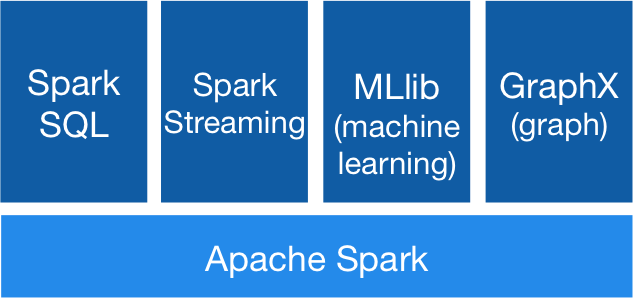
\includegraphics[width=0.5\linewidth]{spark-stack.png}}
    \caption{Zusammensetzung des Spark-Frameworks\cite{spark}}
    \label{fig:sparkstack}
\end{figure}

Beispielhaft für den Spark-Stack seien hier die Bibliotheken MLlib\cite{mllib} und GraphX erwähnt.

MLlib, kurz für Machine Learning Library, umfasst Funktionen wie lineare Regression, den K-Means-Algorithmus, Latent Dirichlet Allocation, Hauptkomponentenanalyse, das für Maschinenlernen benötigte stochastische Gradientenverfahren, u. v. m. Diese Algorithmen können so mit Spark auf riesigen Datenmengen parallel und einfach angewandt werden.

% GraphX
GraphX erweitert Spark-RDDs zu Kanten- und Knoten-RDDs die als Tupel einen Graph beschreiben \cite{graphx}. Auf diesen abgeleiteten Datentypen sind übliche RDD- und Mengenoperationen wie \lstinline!filter!, \lstinline!diff!, u.a. für das Erstellen und Modifizieren von Graphen möglich. Dieser Graph kann z.B. Webseitenrelationen, jeder Link ist eine Kante im Graph, jede Domain ein Knoten, darstellen. Auf diesen Graphen sind mit GraphX parallel Algorithmen wie PageRank oder das Auszählen von Dreiecken in Graphen ausführbar.


% Executor, Masternode
Für kleinere Tests kann Spark local auf einem Computer bzw. Knoten ausgeführt werden:
\begin{lstlisting}
spark-shell --master local[*]
\end{lstlisting}\vspace{-1.5\baselineskip}
In diesem Beispielaufruf der interaktiven Spark-Shell werden so viele Threads genutzt wie es logische Kerne gibt.

Für das Ausführen auf einem Cluster ist jedoch das getrennte Starten von einem Spark Driver (Master) und mindestens einem Executor (Slave, Worker) notwendig. Der Spark-Driver führt das geschriebene Spark-Programm aus und verteilt z.B. parallelisierbare Map-Anweisungen an die Executoren, welche die zugewiesenen Berechnungen durchführen.

\begin{figure}
    \centerline{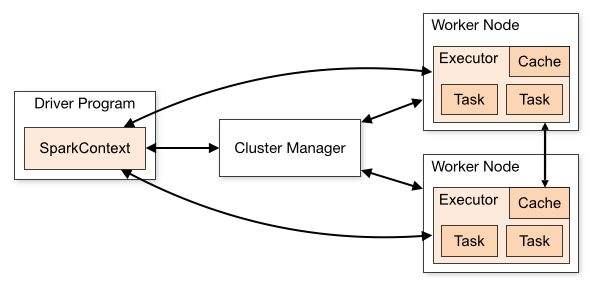
\includegraphics[width=0.8\linewidth]{cluster-overview.png}}
    \caption{Master/Slave-Struktur eines Spark-Clusters\cite{spark}}
    \label{fig:sparkcluster}
\end{figure}

Jeder Executor wird in einer eigenen Java Virtual Machine (JVM), also einem eigenen Prozess ausgeführt. Normalerweise und so auch hier wird für jeden Knoten ein Executor-Prozess gestartet, welcher mit \lstinline!$SPARK_WORKER_CORES! Threads arbeitet. Für den hier vorgestellten Benchmark wird \lstinline!$SPARK_WORKER_CORES! identisch der Anzahl an Grafikkarten auf dem Knoten gewählt, sodass jeder Thread mit einer Grafikkarte arbeiten kann.

%%%%%%%%%%%%%%%%%%%%%%%%%%%%%%%%%%%%%%%%%%%%%%%%%%%%%%%%%%%%%%%%%%%%%%%%%%%%%%%%
\section{Konfiguration von Spark auf einem Slurm-Cluster}
%%%%%%%%%%%%%%%%%%%%%%%%%%%%%%%%%%%%%%%%%%%%%%%%%%%%%%%%%%%%%%%%%%%%%%%%%%%%%%%%

Viele Cluster stellen schon einen Task-Scheduler für Multinutzerumgebungen zur Verfügung, so z.B. das PBS (Portable Batch System) oder SLURM (Simple Linux Utility for Resource Management), um Rechenzeit auf dem Cluster möglichst effizient und gerecht zu verteilen. Außerdem ermöglichen sie das verteilte Starten von Programmen, z.B. jene die mit MPI programmiert wurden. Der für die Benchmarks genutzte Cluster, siehe \autoref{sct:taurus}, arbeitet mit SLURM.

Um Spark nutzen zu können müssen zuerst Master- und Slave-Knoten gestartet werden. Damit alle gleichzeitig gestartet werden, kann Slurms \lstinline!--multi-prog! Option genutzt werden, welche als Argument einen Pfad zu einer Konfigurationsdatei erwartet, in der für jeden Rank ein auszuführendes Programm angegeben werden muss.

Alternativ kann man auch anhand von der Umgebungsvariable \lstinline!SLURM_PROCID! im Skript entweder einen Master-Knoten oder einen Slave-Knoten starten. Letzeres wurde aufgrund der Übersichtlichkeit, d.h. alle Funktionalitäten in einem Skript zu haben, gewählt, siehe Listing~\ref{lst:start_spark_slurm.sh}.

Auf dem Master-Knoten wird der Spark Driver mit
\begin{lstlisting}
"$SPARK_ROOT/bin/spark-class" org.apache.spark.deploy.master.Master \
    --ip $(hostname) --port 7077 --webui-port 8080 &
\end{lstlisting}\vspace{-1.5\baselineskip}
gestartet.
Alle anderen Knoten starten einen Executor-Prozess mit:
\begin{lstlisting}
"$SPARK_ROOT/bin/spark-class" org.apache.spark.deploy.worker.Worker \
    spark://$(scontrol show hostname $SLURM_NODELIST | head -n 1):7077
\end{lstlisting}\vspace{-1.5\baselineskip}
Hierbei wird vorausgesetzt, dass der Masterknoten, also jener für den \lstinline!$SLURM_PROCID=0! ist, der erste Knoten in \lstinline!$SLURM_NODELIST! ist. Dies wurde per assert vom Masterknoten aus auch geprüft und ist bei keinem der rund 50 Versuche fehlgeschlagen.

Wenn Spark gestartet ist, kann sich z.B. mit einer aktiven Eingabeaufforderung an den Master verbunden werden:
\begin{lstlisting}[language=bash]
export MASTER_ADDRESS=spark://$MASTER_IP:7077
spark-shell --master=$MASTER_ADDRESS
\end{lstlisting}\vspace{-1.5\baselineskip}
Die Umgebungsvariable \lstinline!$MASTER_ADDRESS! wird automatisch vom \lstinline!startSpark.sh!-Skript im Quellcodeverzeichnis\cite{scaromare} gesetzt.
